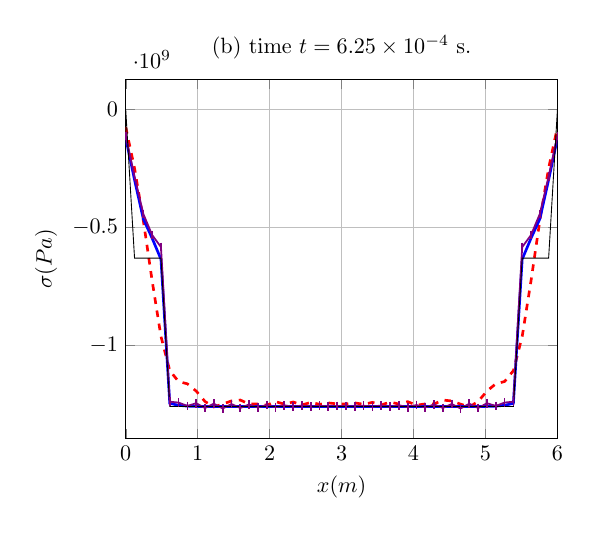
\begin{tikzpicture}[scale=0.8]
\begin{axis}[xlabel=$x (m)$,ylabel=$\sigma (Pa)$,ymajorgrids=true,xmajorgrids=true,legend pos=outer north east,title={(b) time $t = 6.25\times 10^{-4} $ s.},xmin=0.,xmax=6.]
\addplot[Red,very thick,mark=none,dashed] coordinates {(0.0,-74686690.65430246) (0.12244897959183673,-248860978.1693335) (0.24489795918367346,-471505677.3136862) (0.36734693877551017,-727347550.4714894) (0.4897959183673469,-963308331.6520433) (0.6122448979591837,-1108824904.6085515) (0.7346938775510203,-1154837713.915547) (0.8571428571428571,-1164658358.6882505) (0.9795918367346939,-1195327833.6731591) (1.1020408163265305,-1239722495.17177) (1.2244897959183674,-1262625036.5763078) (1.346938775510204,-1250850727.3360605) (1.4693877551020407,-1237335621.1098552) (1.5918367346938775,-1233570784.670482) (1.7142857142857142,-1250022356.590519) (1.836734693877551,-1250064510.2383804) (1.9591836734693877,-1255304260.9119728) (2.0816326530612246,-1240464014.9742188) (2.204081632653061,-1250749408.0219655) (2.326530612244898,-1241771881.0316234) (2.4489795918367347,-1254655253.5739675) (2.571428571428571,-1243386642.1602688) (2.693877551020408,-1251564997.8232079) (2.816326530612245,-1245650942.428049) (2.9387755102040813,-1249901934.3884947) (3.061224489795918,-1249901934.3884926) (3.183673469387755,-1245650942.4280505) (3.306122448979592,-1251564997.8232062) (3.4285714285714284,-1243386642.160271) (3.5510204081632653,-1254655253.5739667) (3.673469387755102,-1241771881.0316243) (3.7959183673469385,-1250749408.0219643) (3.9183673469387754,-1240464014.9742193) (4.040816326530612,-1255304260.911973) (4.163265306122449,-1250064510.238382) (4.285714285714286,-1250022356.59052) (4.408163265306122,-1233570784.670483) (4.530612244897959,-1237335621.1098552) (4.653061224489796,-1250850727.3360612) (4.775510204081632,-1262625036.5763083) (4.8979591836734695,-1239722495.1717708) (5.020408163265306,-1195327833.6731594) (5.142857142857142,-1164658358.688251) (5.26530612244898,-1154837713.915547) (5.387755102040816,-1108824904.6085508) (5.5102040816326525,-963308331.652042) (5.63265306122449,-727347550.4714878) (5.755102040816326,-471505677.3136848) (5.877551020408163,-248860978.16933236) (6.0,-74686690.65430167) };
\addplot[Blue,very thick,mark=none,solid] coordinates {(0.0,-120597397.19248778) (0.12244897959183673,-298539345.15508544) (0.24489795918367346,-464504460.170754) (0.36734693877551017,-546627376.3559334) (0.4897959183673469,-635546108.2543886) (0.6122448979591837,-1247334335.3333962) (0.7346938775510203,-1255980074.5990539) (0.8571428571428571,-1259371705.5275755) (0.9795918367346939,-1260535220.1287405) (1.1020408163265305,-1260885267.5005968) (1.2244897959183674,-1260977777.705495) (1.346938775510204,-1260999265.6570995) (1.4693877551020407,-1261003650.0375175) (1.5918367346938775,-1261004434.5740557) (1.7142857142857142,-1261004557.3391547) (1.836734693877551,-1261004574.0682204) (1.9591836734693877,-1261004576.0419452) (2.0816326530612246,-1261004576.241996) (2.204081632653061,-1261004576.2592359) (2.326530612244898,-1261004576.260481) (2.4489795918367347,-1261004576.260556) (2.571428571428571,-1261004576.2605588) (2.693877551020408,-1261004576.260559) (2.816326530612245,-1261004576.2605588) (2.9387755102040813,-1261004576.260559) (3.061224489795918,-1261004576.2605584) (3.183673469387755,-1261004576.2605586) (3.306122448979592,-1261004576.2605588) (3.4285714285714284,-1261004576.2605581) (3.5510204081632653,-1261004576.2605555) (3.673469387755102,-1261004576.260481) (3.7959183673469385,-1261004576.2592354) (3.9183673469387754,-1261004576.2419953) (4.040816326530612,-1261004576.0419443) (4.163265306122449,-1261004574.06822) (4.285714285714286,-1261004557.3391542) (4.408163265306122,-1261004434.5740552) (4.530612244897959,-1261003650.037517) (4.653061224489796,-1260999265.6570988) (4.775510204081632,-1260977777.7054946) (4.8979591836734695,-1260885267.500596) (5.020408163265306,-1260535220.1287398) (5.142857142857142,-1259371705.5275738) (5.26530612244898,-1255980074.5990536) (5.387755102040816,-1247334335.3333952) (5.5102040816326525,-635546108.2543867) (5.63265306122449,-546627376.3559326) (5.755102040816326,-464504460.1707534) (5.877551020408163,-298539345.15508515) (6.0,-120597397.19248791) };
\addplot[Purple,thick,mark=|,solid] coordinates {(0.0,-111808132.50928691) (0.12244897959183673,-283652980.311345) (0.24489795918367346,-443221012.94130766) (0.36734693877551017,-532712483.6212361) (0.4897959183673469,-583780738.0952947) (0.6122448979591837,-1240572116.142149) (0.7346938775510203,-1244261651.762744) (0.8571428571428571,-1258556998.8403206) (0.9795918367346939,-1246923690.2991939) (1.1020408163265305,-1267582002.156853) (1.2244897959183674,-1248919510.011234) (1.346938775510204,-1269351209.0749319) (1.4693877551020407,-1250347534.9609652) (1.5918367346938775,-1267308507.8062203) (1.7142857142857142,-1252234928.1894917) (1.836734693877551,-1265091742.2400982) (1.9591836734693877,-1254542095.0106862) (2.0816326530612246,-1263677501.5970206) (2.204081632653061,-1255669724.044529) (2.326530612244898,-1262623936.670721) (2.4489795918367347,-1256618647.3458264) (2.571428571428571,-1261747368.978006) (2.693877551020408,-1257589986.0890632) (2.816326530612245,-1260580011.675211) (2.9387755102040813,-1258915831.3187945) (3.061224489795918,-1258915831.3187914) (3.183673469387755,-1260580011.6752121) (3.306122448979592,-1257589986.0890625) (3.4285714285714284,-1261747368.9780068) (3.5510204081632653,-1256618647.3458252) (3.673469387755102,-1262623936.6707222) (3.7959183673469385,-1255669724.0445278) (3.9183673469387754,-1263677501.5970201) (4.040816326530612,-1254542095.0106847) (4.163265306122449,-1265091742.2400992) (4.285714285714286,-1252234928.1894906) (4.408163265306122,-1267308507.80622) (4.530612244897959,-1250347534.9609656) (4.653061224489796,-1269351209.0749316) (4.775510204081632,-1248919510.0112329) (4.8979591836734695,-1267582002.1568534) (5.020408163265306,-1246923690.2991939) (5.142857142857142,-1258556998.8403208) (5.26530612244898,-1244261651.7627428) (5.387755102040816,-1240572116.1421485) (5.5102040816326525,-583780738.0952928) (5.63265306122449,-532712483.6212349) (5.755102040816326,-443221012.9413062) (5.877551020408163,-283652980.3113445) (6.0,-111808132.50928625) };
\addplot[black,thin,mark=none,solid] coordinates {(0.0,-0.0) (0.12244897959183673,-630502288.1302795) (0.24489795918367346,-630502288.1302795) (0.36734693877551017,-630502288.1302795) (0.4897959183673469,-630502288.1302795) (0.6122448979591837,-1261004576.260559) (0.7346938775510203,-1261004576.260559) (0.8571428571428571,-1261004576.260559) (0.9795918367346939,-1261004576.260559) (1.1020408163265305,-1261004576.260559) (1.2244897959183674,-1261004576.260559) (1.346938775510204,-1261004576.260559) (1.4693877551020407,-1261004576.260559) (1.5918367346938775,-1261004576.260559) (1.7142857142857142,-1261004576.260559) (1.836734693877551,-1261004576.260559) (1.9591836734693877,-1261004576.260559) (2.0816326530612246,-1261004576.260559) (2.204081632653061,-1261004576.260559) (2.326530612244898,-1261004576.260559) (2.4489795918367347,-1261004576.260559) (2.571428571428571,-1261004576.260559) (2.693877551020408,-1261004576.260559) (2.816326530612245,-1261004576.260559) (2.9387755102040813,-1261004576.260559) (3.061224489795918,-1261004576.260559) (3.183673469387755,-1261004576.260559) (3.306122448979592,-1261004576.260559) (3.4285714285714284,-1261004576.260559) (3.5510204081632653,-1261004576.260559) (3.673469387755102,-1261004576.260559) (3.7959183673469385,-1261004576.260559) (3.9183673469387754,-1261004576.260559) (4.040816326530612,-1261004576.260559) (4.163265306122449,-1261004576.260559) (4.285714285714286,-1261004576.260559) (4.408163265306122,-1261004576.260559) (4.530612244897959,-1261004576.260559) (4.653061224489796,-1261004576.260559) (4.775510204081632,-1261004576.260559) (4.8979591836734695,-1261004576.260559) (5.020408163265306,-1261004576.260559) (5.142857142857142,-1261004576.260559) (5.26530612244898,-1261004576.260559) (5.387755102040816,-1261004576.260559) (5.5102040816326525,-630502288.1302795) (5.63265306122449,-630502288.1302795) (5.755102040816326,-630502288.1302795) (5.877551020408163,-630502288.1302795) (6.0,-0.0) };
%\legend{usl 1ppc,dgmpm 1ppc (ep solver),dgmpm 1ppc (ac solver),exact}
\end{axis}
\end{tikzpicture}
%%% Local Variables:
%%% mode: latex
%%% TeX-master: "../../mainManuscript"
%%% End:
